% Harus dimuat terlebih dahulu, digunakan agar file PDF memiliki format karakter yang benar.
% Untuk informasi lebih lanjut, lihat https://ctan.org/pkg/cmap.
\RequirePackage{cmap}

% Format dokumen sebagai paper konferensi menggunakan aturan IEEEtran terbaru (v1.8b).
% Untuk informasi lebih lanjut, lihat http://www.michaelshell.org/tex/ieeetran/.
\documentclass[conference]{IEEEtran}[2015/08/26]

% Format encoding font dan input menjadi 8-bit UTF-8.
\usepackage[T1]{fontenc}
\usepackage[utf8]{inputenc}

% Format bahasa menjadi bahasa german dan inggris.
\usepackage[indonesian]{babel}

% Digunakan untuk tujuan demonstrasi.
\usepackage{mwe}

% Digunakan untuk menampilkan font dengan style yang lebih baik.
\usepackage[zerostyle=b,scaled=.75]{newtxtt}

% Digunakan untuk menampilkan tabel dengan style yang lebih baik.
\usepackage{booktabs}

% Digunakan untuk menampilkan gambar pada dokumen.
\usepackage{graphicx}

% Digunakan untuk menampilkan potongan kode.
\usepackage{listings}
\lstset{
  basicstyle=\ttfamily,
  columns=fixed,
  basewidth=.5em,
  xleftmargin=0.5cm,
  captionpos=b
}

% Digunakan agar backticks (`) dapat dirender pada PDF.
% Untuk informasi lebih lanjut, lihat https://tex.stackexchange.com/a/341057/9075.
\usepackage{upquote}

% Digunakan untuk menyeimbangkan bagian akhir dokumen dengan dua kolom.
\usepackage{balance}

% Digunakan untuk menampilkan pustaka.
\usepackage[square,comma,numbers,sort&compress]{natbib}

% Mengubah format ukuran teks pada natbib.
\renewcommand{\bibfont}{\normalfont\footnotesize}

% Menambah nama penulis ketika menggunakan perintah \citet.
% Untuk informasi lebih lanjut, lihat https://tex.stackexchange.com/a/76075/9075.
\usepackage{etoolbox}
\makeatletter
\patchcmd{\NAT@test}{\else \NAT@nm}{\else \NAT@hyper@{\NAT@nm}}{}{}
\makeatother

% Digunakan untuk melakukan linewrap pada pustaka dengan url yang panjang
% jika terdapat hyphens
\usepackage[hyphens]{url}

% Digunakan untuk menambah hyperlink pada referensi.
\usepackage{hyperref}

% Menonaktifkan warna dan bookmark pada hyperref.
\hypersetup{hidelinks,
  colorlinks=true,
  allcolors=black,
  pdfstartview=Fit,
  breaklinks=true
}

% Digunakan untuk membenarkan hyperref pada gambar.
\usepackage[all]{hypcap}

% Digunakan untuk menampilkan beberapa gambar
\usepackage[caption=false,font=footnotesize]{subfig}

\usepackage{stfloats}

% Tambahkan format tanda hubung yang benar di sini
\hyphenation{
  ro-ket
  me-ngem-bang-kan
  per-hi-tu-ngan
}

\begin{document}

  % Ubah kalimat berikut sesuai dengan judul penelitian.
\title{Estimasi Umur, Gender dan Ras menggunakan \emph{Convolutional Neural Network} Berbasis Citra Wajah} 


% Ubah kalimat-kalimat berikut sesuai dengan nama, institusi, alamat dan kontak penulis.
\author{
  \IEEEauthorblockN{Fathullah Auzan Setyo Laksono}
  \IEEEauthorblockA{Departemen Teknik Komputer\\
    Fakultas Teknologi Elektro\\
    dan Informatika Cerdas\\
    Institut Teknologi Sepuluh Nopember\\
    Surabaya, Indonesia 60111\\
    fathullah.18072@mhs.its.ac.id}

  \and
  \IEEEauthorblockN{Reza Fuad Rachmadi}
  \IEEEauthorblockA{Departemen Teknik Komputer\\
    Fakultas Teknologi Elektro\\
    dan Informatika Cerdas\\
    Institut Teknologi Sepuluh Nopember\\
    Surabaya, Indonesia 60111\\
    fuad@its.ac.id}

  \and
  \IEEEauthorblockN{Dr. Eko Mulyanto Yuniarno}
  \IEEEauthorblockA{Departemen Teknik Komputer\\
    Fakultas Teknologi Elektro\\
    dan Informatika Cerdas\\
    Institut Teknologi Sepuluh Nopember\\
    Surabaya, Indonesia 60111\\
    ekomulyanto@ee.its.ac.id}
}



% Digunakan untuk menampilkan judul dan deskripsi penulis.
\maketitle

  % Mengubah keterangan `Abstract` ke bahasa indonesia.
% Hapus bagian ini untuk mengembalikan ke format awal.
\renewcommand\abstractname{Abstrak}

\begin{abstract}

  % Ubah paragraf berikut sesuai dengan abstrak dari penelitian.
  Fitur wajah seperti identifikasi umur, gender dan etnik dapat sangat berguna 
  dalam banyak pengimplementasian ilmu seperti pengamatan visual, diagnosa medis, 
  sistem interaksi komputer manusia, biometric, pengumpulan informasi, penegakan 
  hukum, pemasaran dan banyak lainnya. Dimana sebagian besar data mengenai fitur 
  wajah tersebut masih diambil secara manual melalui survei ataupun pengamatan 
  pada banyak individu. Berdasarkan World Population Clock pada websitenya, di 
  dunia terdapat lebih dari 7 miliar orang yang tersebar di berbagai macam pulau 
  dan benua. Jumlah tersebut masih terus bertambah sampai sekarang. Dimana di 
  setiap benua dan negara tersebut terdapat berbagai karakteristik dan ciri 
  manusia yang berbeda dengan kata lain Etnik yang berbeda-beda. Dengan banyaknya 
  jumlah penduduk dan keberagamannya tersebut, jika data fitur wajah diambil 
  secara manual akan memakan waktu dan tenaga yang banyak. Oleh karena itu perlu 
  dibuat suatu sistem yang dapat mengestimasi umur, gender dan etnik serta 
  menyimpan penghitungan datanya untuk mempermudah pengumpulan data. Dimana 
  kamera akan menangkap gambar dari seseorang dan dilakukan proses estimasi 
  umur, gender dan etnik yang kemudian datanya disimpan untuk digunakan kedepannya.

\end{abstract}

% Mengubah keterangan `Index terms` ke bahasa indonesia.
% Hapus bagian ini untuk mengembalikan ke format awal.
\renewcommand\IEEEkeywordsname{Kata kunci}

\begin{IEEEkeywords}

  % Ubah kata-kata berikut sesuai dengan kata kunci dari penelitian.
  \emph{CNN}, Umur, Gender, Ras, Citra, Wajah.

\end{IEEEkeywords}


  % Ubah bagian berikut sesuai dengan konten-konten yang akan dimasukkan pada dokumen
  % Ubah judul dan label berikut sesuai dengan yang diinginkan.
\section{Pendahuluan}
\label{sec:pendahuluan}

% Ubah paragraf-paragraf pada bagian ini sesuai dengan yang diinginkan.

Umur, gender dan etnik merupakan beberapa hal penting dalam wajah yang menentukan bagaimana seorang 
individu berinteraksi sosial. Setiap bahasa di dunia memiliki panggilan kehormatan yang berbeda-beda 
untuk pria dan wanita, perbedaan umur juga dapat menentukan bagaimana seseorang harus bersikap dengan 
orang yang lebih muda ataupun dengan yang lebih tua, sedangkan etnik juga dapat menentukan cara berbahasa 
dan berperilaku pada seseorang. Kebiasaan dan sikap tersebut sebagian besar tergantung pada kemampuan 
seseorang dalam memperkirakan atau mengestimasi individu tersebut melalui penampakan gender, umur dan 
etnik. Dimana identitas, ekspresi, gender, umur dan etnik disebut dengan fitur dalam wajah. \par
Selain itu, fitur dalam wajah juga sering digunakan di berbagai bidang, seperti di kepolisian untuk 
mencari pelaku tindak kriminal yang mengidentifkasi pelaku dari wajah. diagnosa medis yang menggunakan 
wajah untuk menentukan penanganan yang cocok untuk pasien. Di dunia bisnis fitur wajah juga digunakan 
dalam pembagian target pasar untu lebih meningkatkan proses bisnis. \par
Hal ini membuat identifikasi umur, gender dan etnik dapat sangat berguna dalam banyak pengimplementasian 
ilmu seperti pengamatan visual, diagnosa medis, sistem interaksi komputer manusia, biometrik, pengumpulan 
informasi, penegakan hukum, pemasaran dan banyak lainnya. Dimana sebagian besar data mengenai fitur wajah 
tersebut masih diambil secara manual melalui survei ataupun pengamatan pada banyak individu. \par
Berdasarkan \textit{World Population Clock} pada websitenya, di dunia terdapat lebih dari 7 miliar orang yang 
tersebar di berbagai macam pulau dan benua. Jumlah tersebut masih terus bertambah sampai sekarang \citep{Worldometer}.
Dimana di setiap benua dan negara tersebut terdapat berbagai karakteristik dan ciri manusia yang berbeda 
dengan kata lain Etnik yang berbeda-beda \citep{Infoplease}. Dengan banyaknya jumlah penduduk dan keberagamannya tersebut, 
jika data fitur wajah diambil secara manual akan memakan waktu dan tenaga yang banyak.

  % Ubah judul dan label berikut sesuai dengan yang diinginkan.
\section{Penelitian Terkait}
\label{sec:penelitianterkait}

% Ubah paragraf-paragraf pada bagian ini sesuai dengan yang diinginkan.

Beberapa penelitian lain pernah dilakukan seperti yang dirumuskan oleh \citet{newton1687} bahwa \lipsum[5]
Hasil tersebut kemudian menjadi persamaan \ref{eq:hukumpertama}.

% Contoh pembuatan persamaan ilmiah.
\begin{equation}
  \label{eq:hukumpertama}
  \sum \mathbf{F} = 0\; \Leftrightarrow\; \frac{\mathrm{d} \mathbf{v} }{\mathrm{d}t} = 0.
\end{equation}

\lipsum[6-7]

  % Ubah judul dan label berikut sesuai dengan yang diinginkan.
\section{Desain dan Implementasi Sistem}
\label{sec:arsitektur}

% Ubah paragraf-paragraf pada bagian ini sesuai dengan yang diinginkan.

Penelitian ini dilaksanakan sesuai dengan desain sistem berikut dengan implementasinya. Desain sistem merupakan konsep dari
pembuatan dan perancangan infrastruktur dan kemudian diwujudkan dalam bentuk blok-blok alur yang harus dikerjakan. Pada 
bagian implementasi merupakan pelaksanaan teknis untuk setiap blok pada desain sistem. Gambar 3.2 menunjukkan bagan umum 
metodologi sistem.
\begin{figure} [ht]
  \centering
  % Ubah sesuai dengan nama file gambar dan ukuran yang akan digunakan.
  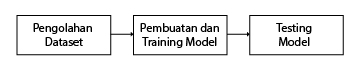
\includegraphics[width=0.5\textwidth]{gambar/metodologi.jpg}

  % Ubah sesuai dengan keterangan gambar yang diinginkan.
  \caption{Diagram blok metodologi.}
  \label{fig:metodologi}
\end{figure}

Pada tahap awal, dataset yang digunakan akan dicek dan dibagi berdasarkan \textit{training}, \textit{validation} dan 
\textit{testing}, serta menyiapkan dataset untuk digunakan pada pembuatan model nantinya. Kemudian 
memilih model atau arsitektur \textit{Convolutional Neural Network} atau \textit{CNN} yang tepat sesuai dengan UTKFace 
dataset yang telah disediakan sebelumnya dan membangun model untuk keperluan training.
Di tahap training, dataset akan digunakan untuk melatih komputer dengan cara mengolah gambar dan anotasi 
yang telah dibuat sehingga terbentuk pola atau karakteristik dari masing masing kelas yang akan 
menjadi bahan pertimbangan komputer dalam mencapai sebuah keputusan atau melakukan prediksi. 
Proses training akan dilakukan menggunakan \textit{Covolutional Neural Network} atau \textit{CNN} pada citra wajah 
yang diberikan. Model yang sudah jadi akan dievaluasi dan dilakukan testing dengan dataset
yang telah disediakan. Selain itu juga membuat prototype sistem sebagai gambaran implementasi penggunaan model.

\subsection{Pengolahan Dataset}
\label{subsec:pengolahandataset}

Dataset yang digunakan dalam Tugas Akhir ini adalah dataset wajah UTKFace dengan rentan umur dari 0 hingga 116 tahun. 
Terdiri atas lebih dari 20.000 gambar wajah dengan anotasi umur, jenis kelamin dan etnik. Sebelum menggunakannya,
dataset ini akan melalui fase pengolahan terlebih dahulu dengan membagi, menyesuaikan ukuran dan mengatur jumlah batch
yang digunakan dalam pembuatan model.  
Dalam dataset UTFace label sudah tersedia pada format nama dari masing-masing gambarnya yaitu umur, gender dan ras.

% Contoh input gambar pada kolom.
\begin{figure} [ht]
  \centering
  % Ubah sesuai dengan nama file gambar dan ukuran yang akan digunakan.
  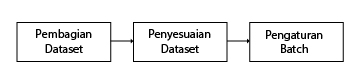
\includegraphics[width=0.5\textwidth]{gambar/dataset.jpg}

  % Ubah sesuai dengan keterangan gambar yang diinginkan.
  \caption{Urutan Pengolahan Dataset}
  \label{fig:pengolahandataset}
\end{figure}

Dikarenakan label umur dari dataset menggunakan umur dalam bentuk angka, untuk menyesuaikan
kelas yang sesuai untuk model nantinya, harus dikategorikan menjadi Balita, Anak, Remaja, Dewasa, Lansia dan Manula. 
Persebaran masing-masing gambar berdasarkan umur, gender dan ras dapat dilihat pada tabel.

\begin{table}
  \caption{Persebaran Umur}
  \label{tab:persebaranumur}
  \centering
  \begin{tabular}{ll}
    \toprule
    \textbf{Rentang Umur} & \textbf{Jumlah} \\
    \midrule
    Balita           & 2363           \\
    Anak             & 920            \\ 
    Remaja           & 4354           \\ 
    Dewasa           & 10457          \\ 
    Lansia           & 3912           \\ 
    Manula           & 1699           \\
    \bottomrule
  \end{tabular}
\end{table}

\begin{table}
  \caption{Persebaran Gender}
  \label{tab:persebarangender}
  \centering
  \begin{tabular}{ll}
    \toprule
    \textbf{Gender} & \textbf{Jumlah} \\
    \midrule
    Pria           & 12391           \\
    Wanita         & 11314           \\
    \bottomrule
  \end{tabular}
\end{table}

\begin{table}
  \caption{Persebaran Ras}
  \label{tab:persebaranras}
  \centering
  \begin{tabular}{ll}
    \toprule
    \textbf{Ras} & \textbf{Jumlah} \\
    \midrule
    White           & 10078           \\
    Black           & 4526            \\
    Indian          & 3975            \\
    Asian           & 3434            \\
    Other           & 1692            \\
    \bottomrule
  \end{tabular}
\end{table}

Selanjutnya dataset akan dibagi menjadi Training, Validation dan Testing untuk memastikan keakuratan model dengan tidak menggunakan dataset 
yang sama pada setiap tahapannya. Untuk pembagiannya, pada tahap training akan menggunakan setengah 
dari total dataset yang ada, tahap validation menggunakan sebesar 0.2 dari total dataset dan pada 
testing menggunakan 0.3 dari total dataset yang ada.

\begin{table}
  \caption{Pembagian Dataset}
  \label{tab:pembagiandataset}
  \centering
  \begin{tabular}{ll}
    \toprule
    \textbf{Pembagian} & \textbf{Jumlah} \\
    \midrule
    Training           & 11615          \\
    Validation         & 4978            \\
    Testing            & 7112            \\
    \bottomrule
  \end{tabular}
\end{table}

Ukuran Dataset yang ada diubah menjadi 198 x 198 pixel dan mengubah format dari gambar menjadi format array dan membaginya dengan 255 agar
format arraynya menjadi rentang 0 sampai 1. Terakhir untuk memasukan dataset ke dalam model, akan dibuat data generator yang akan 
memasukkan gambar dan label yang telah disimpan ke dalam model dan membaginya proses pemasukan gambar berdasarkan ukuran batch 
untuk menghemat memory yang digunakan dengan tidak memuat semua dataset dalam satu waktu.


\subsection{Pembuatan dan Training Model}
\label{subsec:model}

Setelah dataset siap digunakan untuk training, selanjutnya menentukan arsitektur model mana yang cocok untuk digunakan.
Terdapat beberapa arsitektur \textit{Convolutional Neural Network} yang sudah terbukti cocok digunakan dalam kasus 
klasifikasi dengan input gambar. Dalam hal ini arsitektur yang digunakan adalah \textit{ResNet50, VGG16, Inception V3} dan \textit{EfficienNet B0} 
dengan mencoba \textit{weight} dan \textit{optimizer} yang berbeda-beda. Selain menggunakan arsitektur model yang sudah ada, dilakukan 
juga percobaan menggunakan arsitektur sederhana \textit{Convolutional Neural Network} untuk nantinya dibandingkan dengan arsitektur 
yang ada. \par

Metric merupakan indikator yang menunjukkan apakah model yang ditraining menghasilkan prediksi yang bagus atau tidak. Ada berbagai jenis 
metric yang bisa digunakan, namun di sini hanya menggunakan accuracy dan loss untuk mengitung tingkat keberhasilan model yang digunakan. 
Untuk penghitungan metricnya akan dilakukan sebanyak dua kali yaitu pada saat Training dan Validation yang menggunakan dataset yang telah 
dibagi sebelumnya. Kemudian membandingkan hasil accuracy dan loss Training dengan Validation. \par

Selanjutnya pada proses traning mengatur input dari dataset yang akan diberikan ke model, dimana diatur menjadi 198 x 198 dengan jumlah channel 3. 
Yang kemudian akan dilakukan training menggunakan arsitektur CNN \textit{ResNet50, VGG16, Inception V3} dan \textit{EfficienNet B0} serta arsitektur CNN 
sederhana yang telah dibuat sebelumnya. Setelah itu diberi layer terakhir berupa Dense Layer untuk memberikan output prediksinya berupa 
umur, gender dan ras. 

\begin{figure} [ht]
  \centering
  % Ubah sesuai dengan nama file gambar dan ukuran yang akan digunakan.
  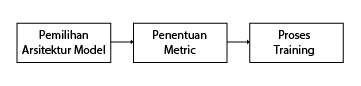
\includegraphics[width=0.5\textwidth]{gambar/model.jpg}

  % Ubah sesuai dengan keterangan gambar yang diinginkan.
  \caption{Urutan Pembuatan Dataset}
  \label{fig:model}
\end{figure}

\subsection{Testing Model}
\label{subsec:testing}

Pada tahap ini testing dilakukan dengan tiga tahap seperti pada Gambar \ref{fig:testing}.
\begin{figure} [ht]
  \centering
  % Ubah sesuai dengan nama file gambar dan ukuran yang akan digunakan.
  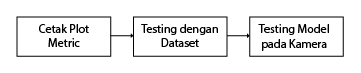
\includegraphics[width=0.4\textwidth]{gambar/testing.jpg}

  % Ubah sesuai dengan keterangan gambar yang diinginkan.
  \caption{Urutan Pelasksanaan Testing}
  \label{fig:testing}
\end{figure}


Setelah masing-masing proses training selesai, nilai dari loss dan akurasi pada masing-masing kelas akan dicetak berdasarkan jumlah epochnya 
menggunakan diagram garis. Dalam diagram tersebut yang perlu diperhatikan adalah kesesuaian tingkat akurasi dan loss pada diagram sudah sesuai 
atau belum. Kemudian melakukan testing dengan dataset yang telah disediakan sebelumnya menggunakan fungsi \textit{classification report} yang akan 
menghitung nilai precision, recall dan f1-score nya sebagai acuan keakuratan model. Selanjutnya model akan dicoba pada prototype sistem untuk 
memberikan gambaran penggunaan model pada kasus nyata. Sistem dibuat dalam bentuk aplikasi website yang dapat mendeteksi umur, gender dan ras 
melalui foto wajah dan melalui webcam yang kemudian difoto untuk di prediksi umur, gender dan rasnya.

\begin{figure} [ht]
  \centering
  % Ubah sesuai dengan nama file gambar dan ukuran yang akan digunakan.
  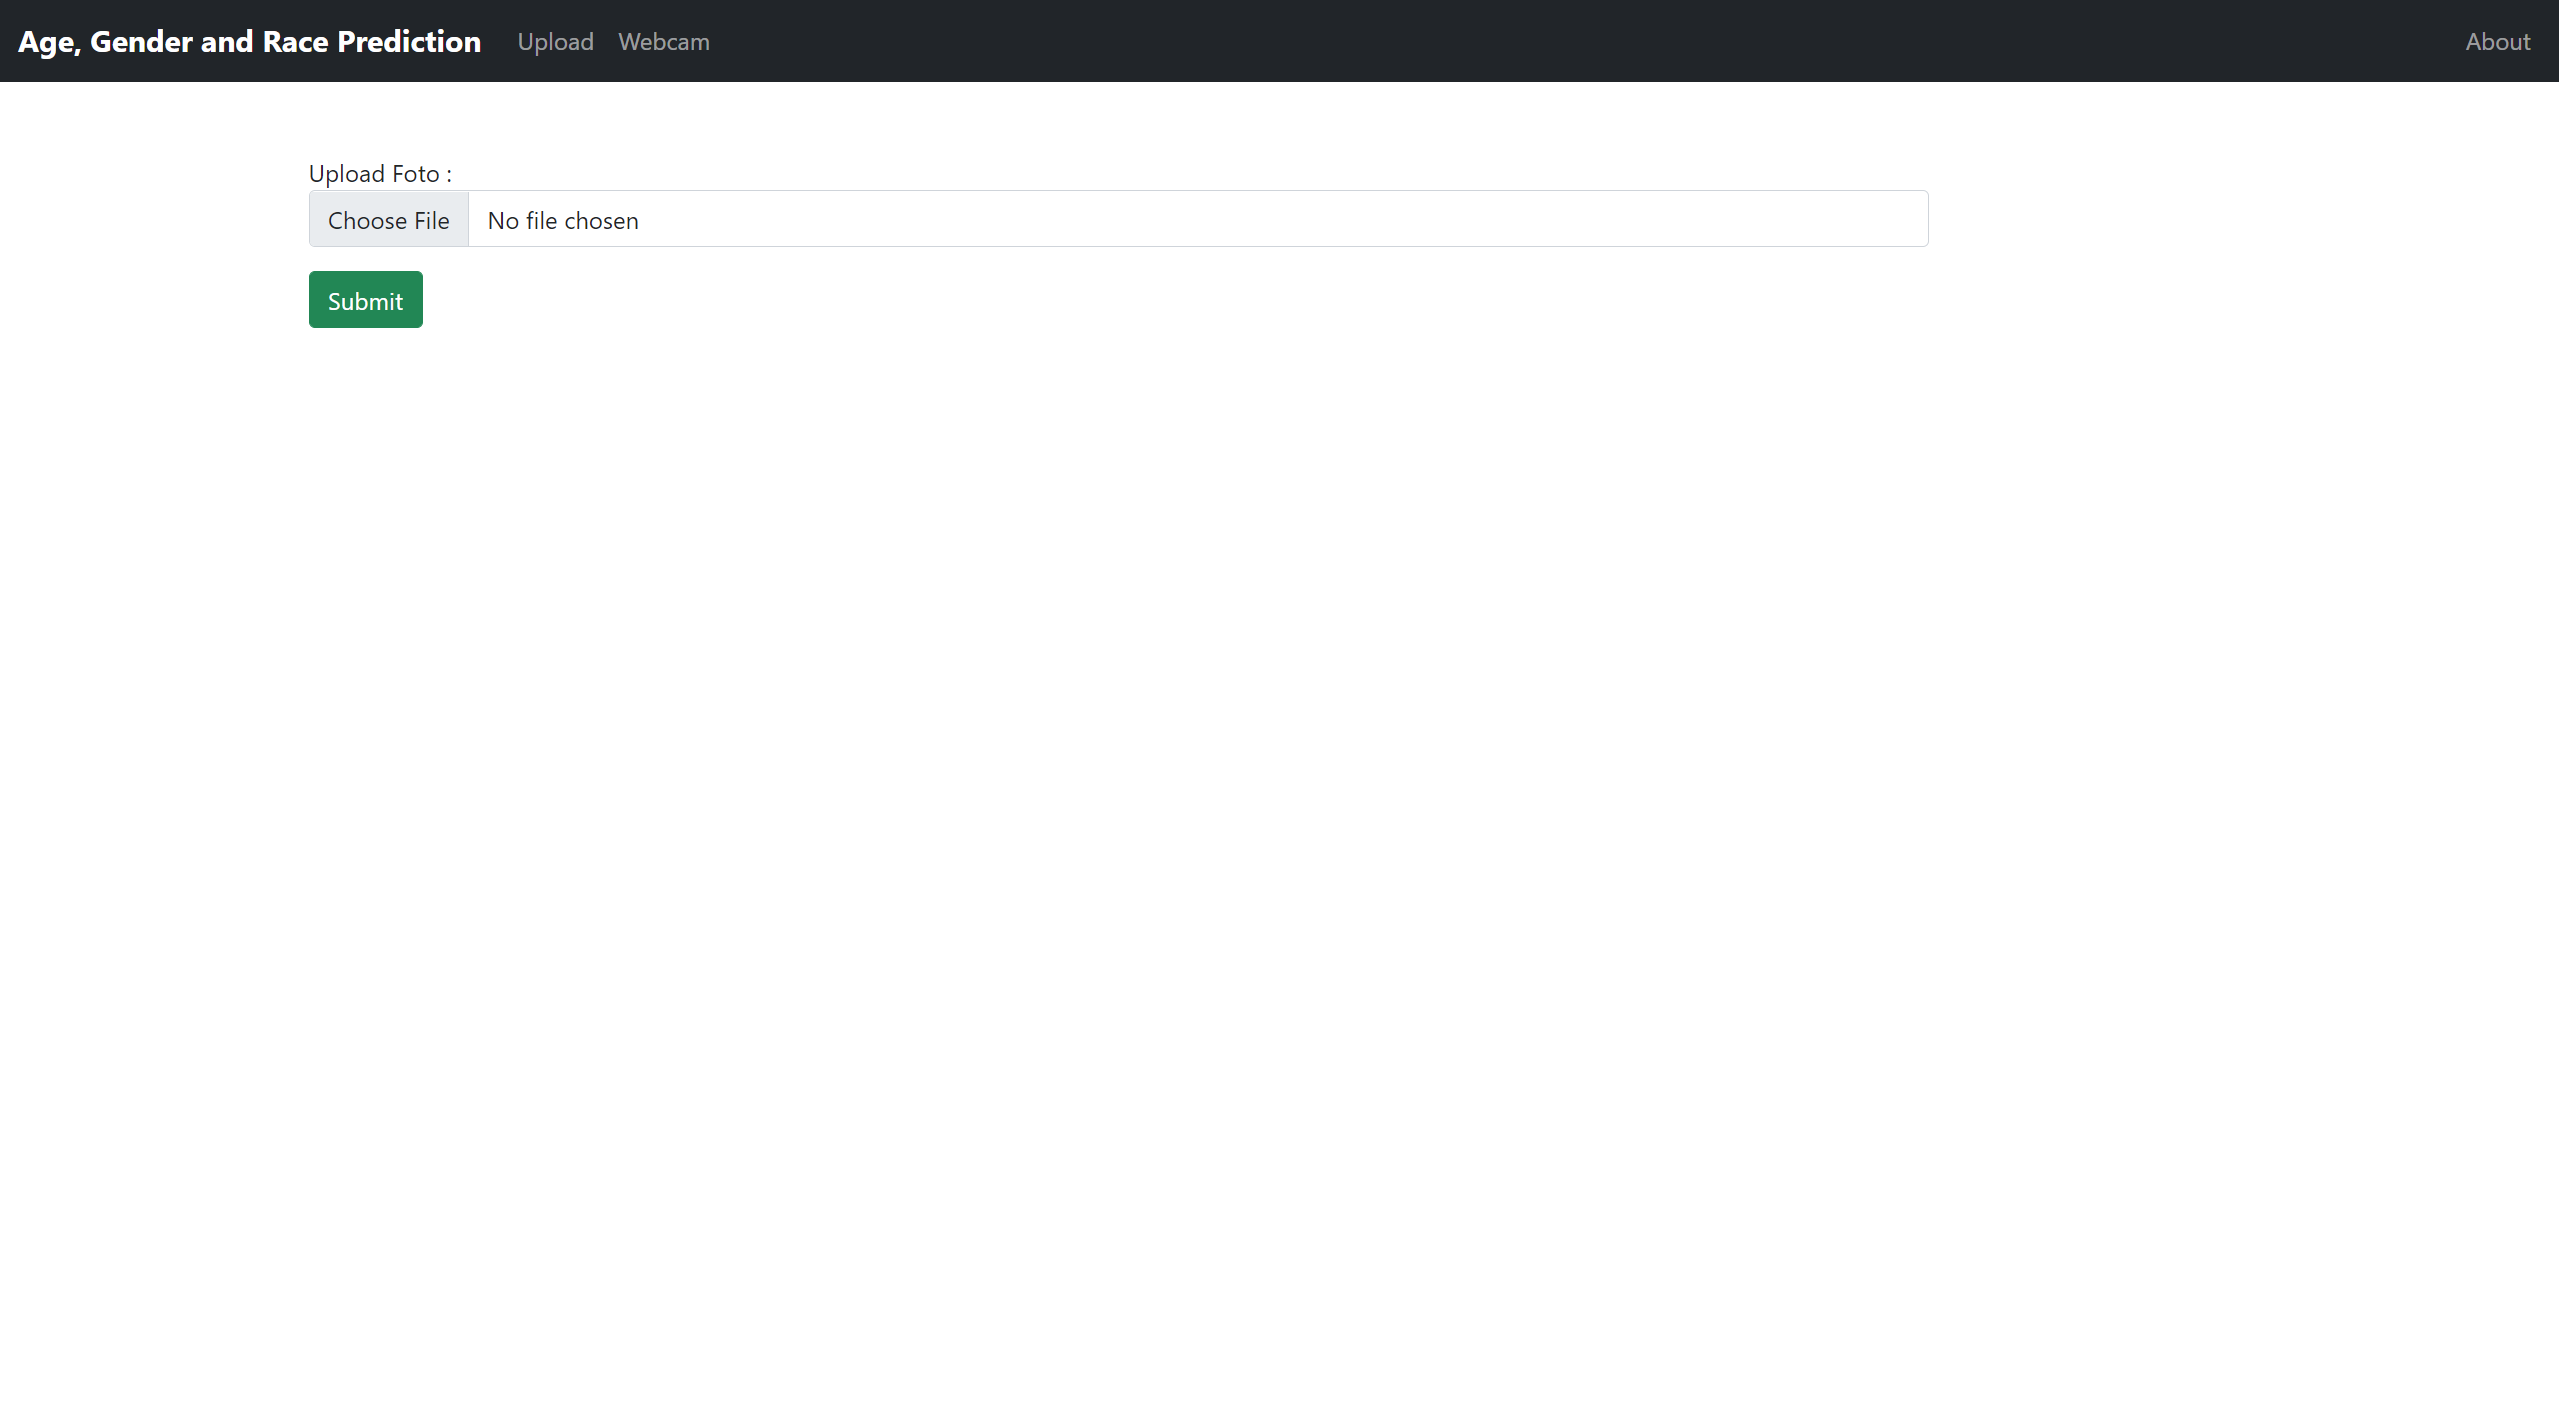
\includegraphics[width=0.4\textwidth]{gambar/webKosong.png}

  % Ubah sesuai dengan keterangan gambar yang diinginkan.
  \caption{Tampilan Web dengan inputan memilih dari folder}
  \label{fig:webupload}
\end{figure}

\begin{figure} [ht]
  \centering
  % Ubah sesuai dengan nama file gambar dan ukuran yang akan digunakan.
  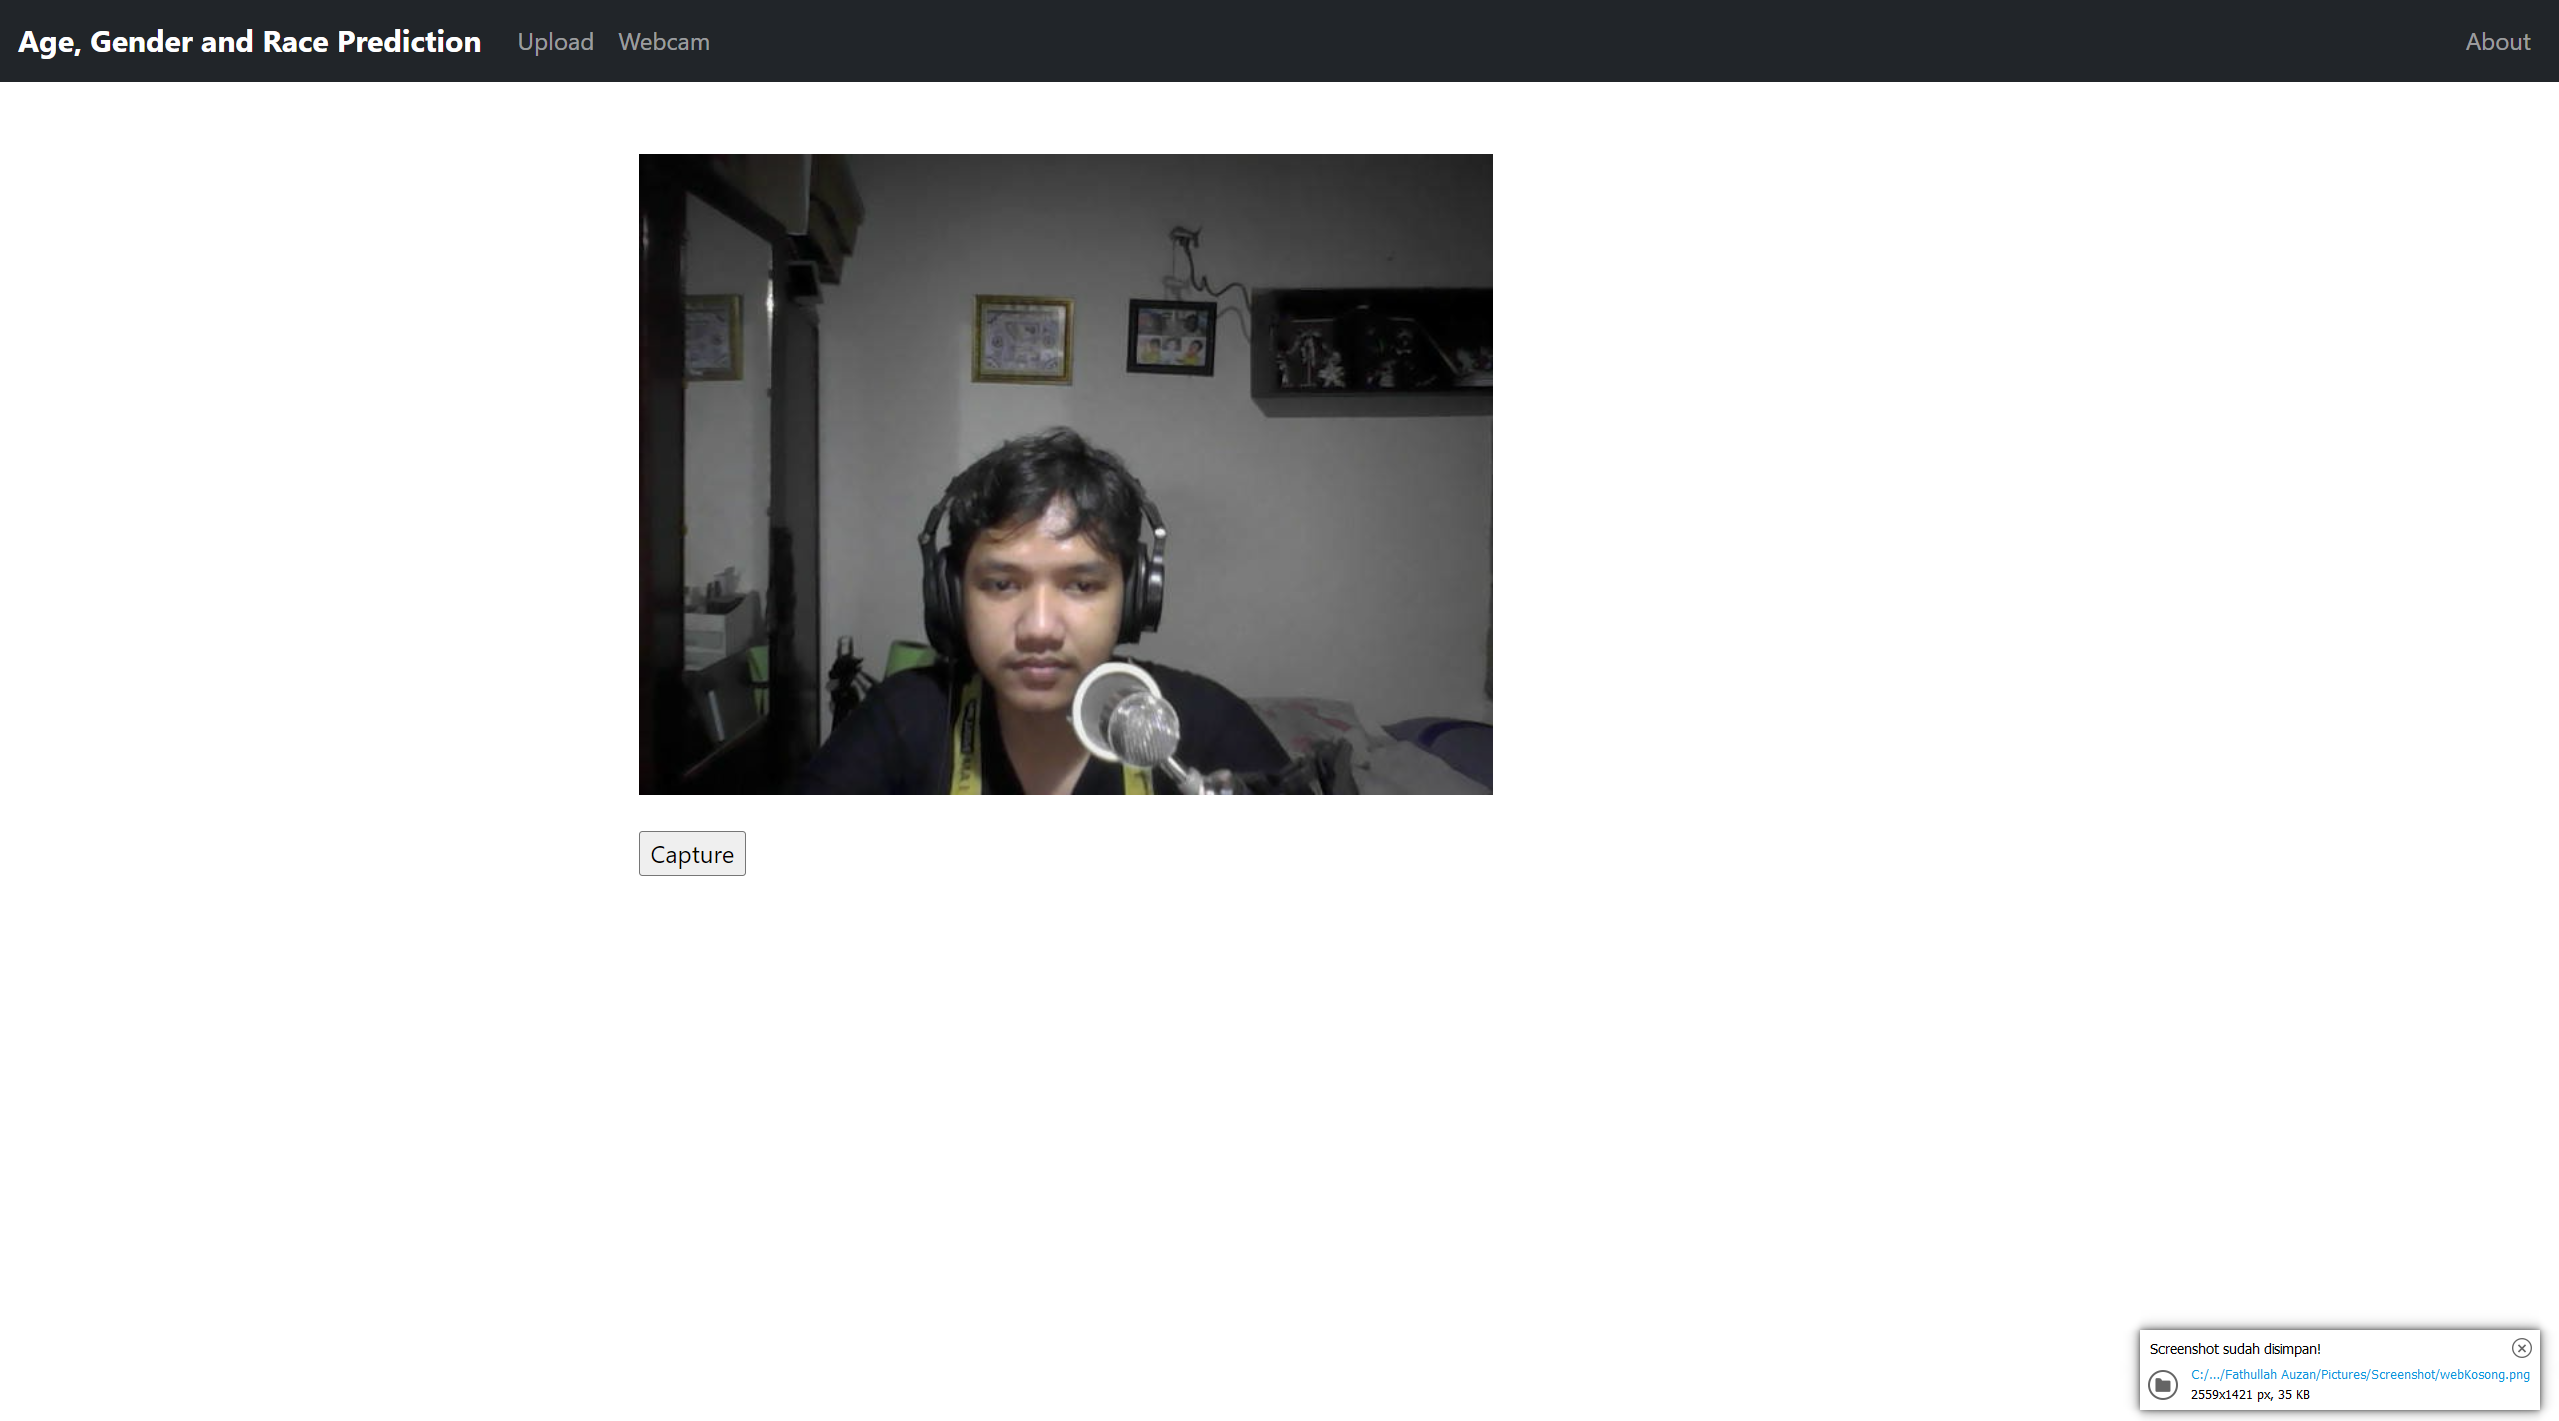
\includegraphics[width=0.5\textwidth]{gambar/WebKosong2.png}

  % Ubah sesuai dengan keterangan gambar yang diinginkan.
  \caption{Tampilan Web dengan inputan foto dari webcam}
  \label{fig:webfoto}
\end{figure}

Dikarenakan model yang dibuat memiliki format tertentu, maka dari itu input foto dari web juga harus diatur terlebih dahulu agar dapat diprediksi dengan 
tepat oleh model. Model yang dibuat menggunakan ukuran foto 198 x 198 pixel, sehingga inputan berupa foto upload maupun dari webcam harus dipotong sesuai ukuran 
tersebut. Selain itu, dalam dataset yang digunakan inputannya hanya sebatas wajah saja tidak terdapat bagian tubuh lainnya. \par

Untuk mengatasi hal tersebut perlu suatu program yang dapat mendeteksi area wajah dalam suatu gambar yaitu dengan menggunakan fungsi Haarcascades pada OpenCV. 
Fungsi tersebut akan mendeteksi area wajah pada gambar, kemudian menyimpan hasil deteksi tersebut ke dalam file foto baru. Hasil potongan wajah 
kemudian diubah ukurannya menjadi 198 x 198 serta diubah ke dalam bentuk array sebelum dilakukan prediksi oleh model. Berikut adalah gambaran tahapan pengolahan 
gambar pada web.

\begin{figure} [ht]
  \centering
  % Ubah sesuai dengan nama file gambar dan ukuran yang akan digunakan.
  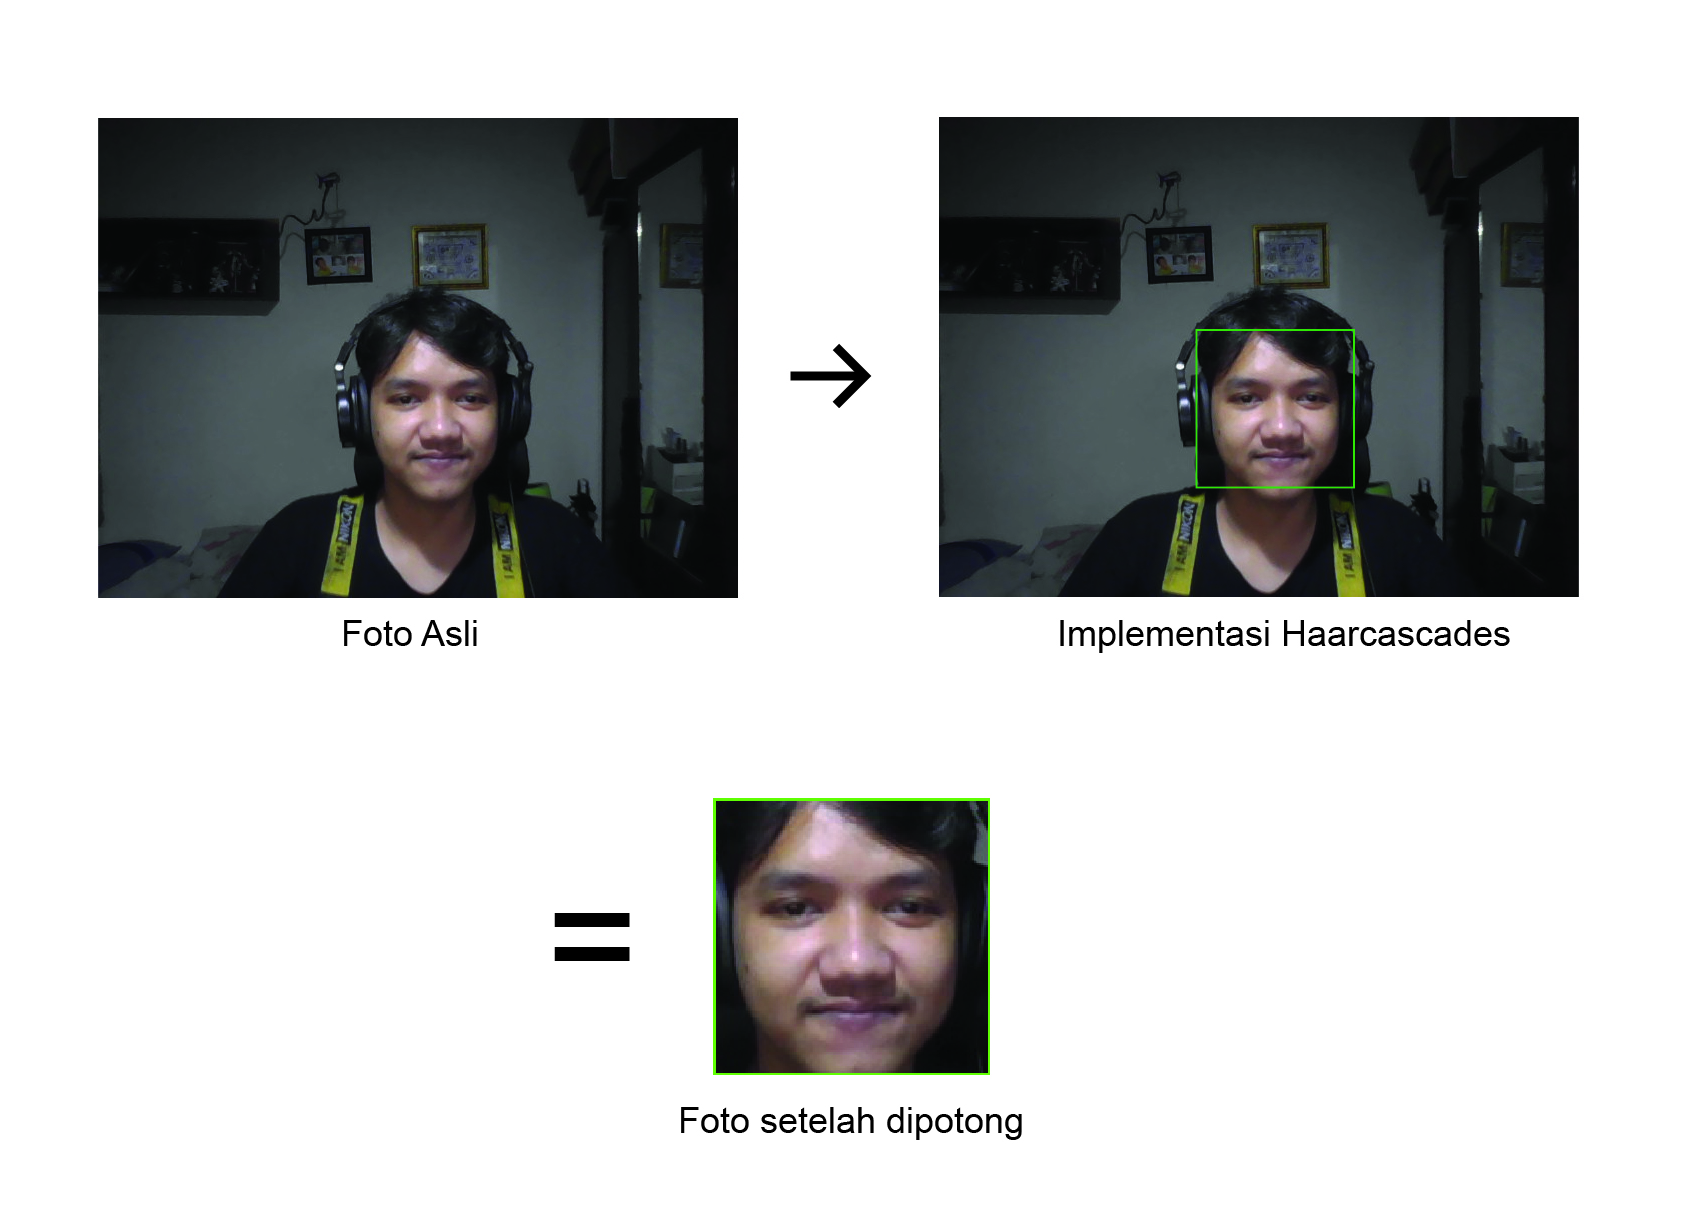
\includegraphics[width=0.5\textwidth]{gambar/preprocessingWeb.jpg}

  % Ubah sesuai dengan keterangan gambar yang diinginkan.
  \caption{Preprocessing pada web}
  \label{fig:preprocessingWeb}
\end{figure}
  % Ubah judul dan label berikut sesuai dengan yang diinginkan.
\section{Lorem ipsum}
\label{sec:loremipsum}

% Ubah paragraf-paragraf pada bagian ini sesuai dengan yang diinginkan.

% Contoh input beberapa gambar pada halaman.
\begin{figure*}
  \centering
  \subfloat[Hasil A]{\includegraphics[width=.4\textwidth]{example-image-a}
    \label{fig:hasila}}
  \hfil
  \subfloat[Hasil B]{\includegraphics[width=.4\textwidth]{example-image-b}
    \label{fig:hasilb}}
  \caption{Contoh input beberapa gambar.}
  \label{fig:hasil}
\end{figure*}

\lipsum[16-18]

% Contoh input potongan kode dari file.
\lstinputlisting[
  language=Python,
  caption={Program perhitungan bilangan prima.},
  label={lst:bilanganprima}
]{program/bilangan-prima.py}

\lipsum[19-20]

  % Ubah judul dan label berikut sesuai dengan yang diinginkan.
\section{Kesimpulan}
\label{sec:kesimpulan}

% Ubah paragraf-paragraf pada bagian ini sesuai dengan yang diinginkan.

\lipsum[21-23]


  % Menampilkan daftar pustaka dengan format IEEE
  \bibliographystyle{IEEEtranN}
  \bibliography{pustaka/pustaka.bib}

  % Menyeimbangkan bagian akhir di kedua kolom
  \balance

\end{document}
